
\section*{Общая характеристика работы}

\newcommand{\actuality}{\underline{\textbf{\actualityTXT}}}
\newcommand{\progress}{\underline{\textbf{\progressTXT}}}
\newcommand{\aim}{\underline{{\textbf\aimTXT}}}
\newcommand{\tasks}{\underline{\textbf{\tasksTXT}}}
\newcommand{\novelty}{\underline{\textbf{\noveltyTXT}}}
\newcommand{\influence}{\underline{\textbf{\influenceTXT}}}
\newcommand{\methods}{\underline{\textbf{\methodsTXT}}}
\newcommand{\defpositions}{\underline{\textbf{\defpositionsTXT}}}
\newcommand{\reliability}{\underline{\textbf{\reliabilityTXT}}}
\newcommand{\probation}{\underline{\textbf{\probationTXT}}}
\newcommand{\contribution}{\underline{\textbf{\contributionTXT}}}
\newcommand{\publications}{\underline{\textbf{\publicationsTXT}}}


{\actuality} Обзор, введение в тему, обозначение места данной работы в
мировых исследованиях и~т.\:п.

Традиционный подход (построение аналитических моделей):
\begin{itemize}
\item  сложная система разбивается на несколько независимых уровней
\item  определяются показатели эффективности каждого уровня
\item  производится построение, валидация и верификация <аналитических> моделей каждого уровня
\item  показатели каждого уровня оптимизируются в модельных сценариях
\item  производится подстройка модели
\end{itemize}


Предлагаемый подход (на основе машинного обучения, генерация фич):
\begin{itemize}
\item  сложная система данных воспринимается как "серый ящик"
\item  определяются показатели эффективности системы в целом 
\item  определяется конечное множество состояний системы
\item  из базовых признаков состояния системы производится порождение составных признаков 
\item  вырабатывается решающее правило
\item  решающее правило и модель принятия решения валидируется экспертами (трактовка результатов)
\end{itemize}

В данной работе предлагается рассмотреть несколько примеров использования машинного обучения в задачах управления инфраструктурой. Далее предлагается обобщить опыт и предложить метод построения и трактовки моделей, полученных при помощи алгоритмов машинного обучения в условиях современной инфраструктуры.


% разнородная по всем
% алгоритмов полно
% основные задачи 



% , можно использовать ссылки на другие
% работы~\cite{Gosele1999161} (если их нет, то в автореферате
% автоматически пропадёт раздел <<Список литературы>>). Внимание! Ссылки
% на другие работы в разделе общей характеристики работы можно
% использовать только при использовании \verb!biblatex! (из-за технических
% ограничений \verb!bibtex8!. Это связано с тем, что одна и та же
% характеристика используются и в тексте диссертации, и в
% автореферате. В последнем, согласно ГОСТ, должен присутствовать список
% работ автора по теме диссертации, а \verb!bibtex8! не умеет выводить в одном
% файле два списка литературы).

% {\progress} 
% Этот раздел должен быть отдельным структурным элементом по
% ГОСТ, но он, как правило, включается в описание актуальности
% темы. Нужен он отдельным структурынм элемементом или нет ---
% смотрите другие диссертации вашего совета, скорее всего не нужен.

{\aim} данной работы является \ldots

Для~достижения поставленной цели необходимо было решить следующие {\tasks}:
\begin{enumerate}
  \item Обзор и анализ существующих алгоритмов управления инфраструктурой на основе оперативных массивов данных
  \item Разработка и исследование методов и алгоритмов управления радио-ресурсами в телекоммуникационных сетях четвертого поколения (4G)
  \item Разработка и исследование методов и алгоритмов управления приоритетом обработки инцидентов на основе оперативных данных устройств железнодорожной автоматики и телемеханики
  \item Экспериментальное исследование характеристик разработанных моделей, обобщение на более широкий класс задач

\end{enumerate}

{\novelty}
\begin{enumerate}
  \item Впервые \ldots
  \item Впервые \ldots
  \item Было выполнено оригинальное исследование \ldots
\end{enumerate}

{\influence} \ldots

{\methods} Для решения задач, поставленных в работе, были использованы основные положения системного анализа, теории информации, теории вероятностей; для проектирования программной системы – методы объектно-ориентированного проектирования и язык UML; для программной реализации алгоритмов и системы – методы структурного, объектно-ориентированного и параллельного программирования.

{\defpositions}
\begin{enumerate}
  \item Способ формирования модели планирования ресурсов телекоммуникационной инфраструктуры, пригодной для применения методов машинного обучения. Децентрализованный метод управления радио-ресурсами в телекоммуникационных сетях четвертого поколения в целях понижения общего уровня интерференции и максимизации суммарной пропускной способности в сети базовых станций.
  \item Алгоритм и режимы работы элементов телекоммуникационной инфраструктуры сетей четвертого поколения, учитывающие требования по  качеству обслуживания пользователей.
  \item Алгоритмов и архитектура управления приоритетом обработки инцидентов на основе оперативных данных устройств железнодорожной автоматики и телемеханики.
  \item Алгоритмов и архитектура управления приоритетом обработки инцидентов на основе оперативных данных устройств железнодорожной автоматики и телемеханики.
\end{enumerate}
% В папке Documents можно ознакомиться в решением совета из Томского ГУ
% в файле \verb+Def_positions.pdf+, где обоснованно даются рекомендации
% по формулировкам защищаемых положений. 

{\reliability} полученных результатов обеспечивается \ldots \ Результаты находятся в соответствии с результатами, полученными другими авторами.


% Внедрение

Программная реализация системы  внедрена... \todo{ссылка на отчет о внедрении}
Программная реализация системы автоматического ранжирования инцидентов внедрена \todo{ссылка на отчет о результатах подконтрольной эксплуатации}

{\probation}
Основные результаты работы докладывались~на:
перечисление основных конференций, симпозиумов и~т.\:п.

{\contribution} Автор принимал активное участие \ldots

%\publications\ Основные результаты по теме диссертации изложены в ХХ печатных изданиях~\cite{Sokolov,Gaidaenko,Lermontov,Management},
%Х из которых изданы в журналах, рекомендованных ВАК~\cite{Sokolov,Gaidaenko}, 
%ХХ --- в тезисах докладов~\cite{Lermontov,Management}.

\ifnumequal{\value{bibliosel}}{0}{% Встроенная реализация с загрузкой файла через движок bibtex8
    \publications\ Основные результаты по теме диссертации изложены в XX печатных изданиях, 
    X из которых изданы в журналах, рекомендованных ВАК, 
    X "--- в тезисах докладов.%
}{% Реализация пакетом biblatex через движок biber
%Сделана отдельная секция, чтобы не отображались в списке цитированных материалов
    \begin{refsection}%
        \printbibliography[heading=countauthornotvak, env=countauthornotvak, keyword=biblioauthornotvak, section=1]%
        \printbibliography[heading=countauthorvak, env=countauthorvak, keyword=biblioauthorvak, section=1]%
        \printbibliography[heading=countauthorconf, env=countauthorconf, keyword=biblioauthorconf, section=1]%
        \printbibliography[heading=countauthor, env=countauthor, keyword=biblioauthor, section=1]%
        \publications\ Основные результаты по теме диссертации изложены в \arabic{citeauthor} печатных изданиях\nocite{qos,globecom}, 
        \arabic{citeauthorvak} из которых изданы в журналах, рекомендованных ВАК\nocite{globecom,ent}, 
        \arabic{citeauthorconf} "--- в тезисах докладов\nocite{globecom,ent}.
    \end{refsection}
}
При использовании пакета \verb!biblatex! для автоматического подсчёта
количества публикаций автора по теме диссертации, необходимо
их здесь перечислить с использованием команды \verb!\nocite!.
    

 % Характеристика работы по структуре во введении и в автореферате не отличается (ГОСТ Р 7.0.11, пункты 5.3.1 и 9.2.1), потому её загружаем из одного и того же внешнего файла, предварительно задав форму выделения некоторым параметрам

%Диссертационная работа была выполнена при поддержке грантов ...

%\underline{\textbf{Объем и структура работы.}} Диссертация состоит из~введения, четырех глав, заключения и~приложения. Полный объем диссертации \textbf{ХХХ}~страниц текста с~\textbf{ХХ}~рисунками и~5~таблицами. Список литературы содержит \textbf{ХХX}~наименование.

%\newpage
\section*{Содержание работы}
Во \underline{\textbf{введении}} обосновывается актуальность диссертационной работы, характеризуются объект и предмет исследования,  формулируются цель и задачи исследования, определяется научная новизна работы, рассматривается степень изученности темы в научной литературе, раскрываются теоретическая значимость и практическая ценность диссертации. Представляются выносимые на защиту основные научные положения, приводятся сведения об апробации полученных результатов и публикациях по теме исследования.


\underline{\textbf{В первой главе}} «Задачи и теоретические аспекты построения автоматизированных систем управления технологическими процессами» обосновывается необходимость построения системы управления технологическими процессами, а также выявляется круг основных проблем  в сфере автоматизации критических процессов с применением методов машинного обучения в эргатических системах.


Обучение с подкреплением - это один из подразделов машинного обучения, в ходе которого обучаемая система (т.н. агент) обучается, взаимодействуя с некоторой модельной средой.
Задача обучения состоит в выработке политики поведения - отображения из состояния агента в принимаемое им действие. Цель обучения - максимизировать финальную скалярную награду (подкрепляющий сигнал).


%\todo{Архитектура, Ядерные методы}
%\todo{The learner is not told which action to take, as in most forms of machine learning, but instead must discover which actions yield the highest reward by trying them. In the most interesting and challenging cases, actions may affect not only the immediate's reward, but also the next situation, and through that all subsequent rewards. These two characteristics-trial-and-error search and delayed reward-are the two most important distinguishing features of reinforcement learning}. \cite{book:963927, sutton1998introduction}

Рассмотрим марковский процесс первого порядка с дискретным временем, в котором вероятность перехода из состояния $x$ в состояние $x'$ под действием $u$ задается как $p_0(x'|x,u)$.  Далее будем рассматривать эволюцию системы на бесконечном горизонте времени, с дисконтированием целевой функции со временем. Введем функцию вознаграждения, зависящую от текущего состояния и применяемого действия как $R(x,u)$ и политику $\pi(u|x)$, определяющую вероятность применения действия в зависимости от текущего состояния $x$.


Предполагая, что политика $\pi$ и начальное состояние системы $x_0$ заданы, вероятность найти систему в состоянии $x_t$ на момент времени $t > 0$ задается следующим выражением:

\begin{equation}
    \label{eq:pxxt}
     p_\pi(x_t|x_0; t) =
     \sum_{u_{0:t−1}, x_{1:t−1}}{
     	\prod_{s=0}^{t-1} {
        	p_0(x_{s+1}|x_s, u_x) \pi(u_s|x_s)
         }
      }
\end{equation}

Таким образом ожидаемое дисконтированное вознаграждение в состоянии $x$, при следовании политике $\pi$ задается следующим выражением:

\begin{equation}
    \label{eq:j_pi}
     J_{\pi}(x) =
     \sum_{s=0}^{\infty}
       \sum_{u', x'}{
          \pi(u'|x')p_\pi(x'|x; s)R(x', u')\gamma^s
        }
\end{equation}
, где $\gamma$ - коэффициент дисконтирования ($0 < \gamma < 1$) и $p_pi(x'|x, 0) = \delta_{x,x'}$. Функция $J_\pi(x)$ называется функцией полезности и определяет ожидаемые выигрыш (вознаграждение) при следовании политике $\pi$. Цель обучения с подкреплением заключается в поиске политики $\pi$, максимизирующей значение $J_\pi(x)$ для всех значений $x$.

Выражение для $J_\pi(x)$ можно переписать в рекурсивном виде:
\begin{equation}
    \label{eq:j_pi_rec}
    \begin{split}
     J_\pi(x) &=
     \sum_u {\pi(u|x)R(x,u)} +
     \sum_{s=1}^{\infty}
       \sum_{u', x'}{
          \pi(u'|x')p_\pi(x'|x; s)R(x', u')\gamma^s
        } \\
        &= \sum_u {\pi(u|x)} \left(
        R(x,u) + \gamma \sum_{x'}{
        		p_0(x'|x; u)J_{\pi}(x')
            }
       		\right)
            \end{split}
\end{equation}

Процесс нахождения $J_\pi(x)$ методом последовательных приближений (см. подробнее~\cite{sutton1998reinforcement}) называется оценкой политики (англ. policy evaluation). После нахождения некоторой оценки  $J_\pi(x)$ мы можем предложить новую политику $\pi'$:

\begin{equation}
    \label{eq:new_policy}
    \begin{split}
    & \pi'(u|x) = \delta_{u,u(x)}, \\
    & u(x) = \argmax_u R(x, u) + \gamma \sum_{x'} p_0(x'|x, u)J_\pi(x')
    \end{split}
\end{equation}

Очевидно, что для новой политики $\pi'$ , будет выполняется выражение $J_{\pi'}(x) \geq J_\pi(x), \forall x$. Может быть показано, что итеративный процедура $$\pi_0 \rightarrow J_{\pi_0} \rightarrow \pi_1 \rightarrow J_{\pi_1} \rightarrow \pi_2 \rightarrow ... \rightarrow J^*$$ сходится  к оптимальному значению $J^*$.

Отметим, что в рассуждениях выше предполагается, что функции $p_0(x'|x,u)$, $R(x,u)$ заранее известны. Перейдем к ситуации, когда это окружение заранее не задано. В этом случае возможно либо выучить эти функции в процессе исследования и перейти к итеративной процедуре поиска оптимальной политики, либо использовать подходы обучения с подкреплением, не предполагающие априорное наличие модели ($p_0(x'|x,u)$, $R(x,u)$) - TD-Lambda \cite{sutton1998reinforcement} или Q-learning~\cite{Watkins:1989}.

В случае, когда $p_0(x'|x,u)$, $R(x,u)$ не известны, оценку дисконтированного вознаграждения для состояния $x$ ($J_\pi(x)$, см. уравнение (\ref{eq:j_pi})) можно получить при помощи сэмплирования:

\begin{equation}
    \label{eq:j_sampling}
   	J_\pi(x) = (1-\alpha)J_\pi(x) + \alpha(r + \gamma J_\pi(x')).
\end{equation}
, где $x$ - текущее состояние, $x'$ - новое состояние после выбора действия $u$ при следовании политике $\pi(u|x)$ и $r$ - наблюдаемая награда.

Уравнение~(\ref{eq:j_sampling}) соответствует ~\cite{sutton1998reinforcement} алгоритму TD(0). Отметим, что, применяя этот подход, перед выбором новой стратегии $\pi'$ требуется дождаться схождения алгоритма. Если же на каждой итерации менять политику $\pi'$ согласно уравнению (\ref{eq:new_policy}), получается другой подход, известный под названием Actor-Critic (см.~\cite{actor_critic}).

Более элегантный способ вычисления оптимальной политики без модели ($p_0(x'|x,u)$, $R(x,u)$) был предложен \cite{Watkins:1989} К. Ваткинсом. Обозначим как $Q(x, u)$ ожидаемое значение функции полезности состояния $x$ при выполнении действия $u$ и дальнейшем следовании оптимальной политике:

\begin{equation}
    \label{eq:q_learning_definition}
    \begin{split}
      & Q(x, u) = R(x, u) + \gamma \sum_{x'} {
          p_0(x'|x, u) \max_{u'} Q(x', u')
       }
       \\
      & J^{∗}(x) = \max_{u} Q(x,u)
     \end{split}
\end{equation}

В стохастическом окружении и при использовании онлайн-обучения уравнение (\ref{eq:q_learning_definition}) приобретает следующий вид:

\begin{equation}
    \label{eq:q_learning_online_stochastic}
    Q(x, u) = Q(x, u) + \alpha(R(x, u) + \gamma max_{u'} Q(x', u') − Q(x, u))
\end{equation},
где $\alpha$ - коэффициент, определяющий скорость обучения, $\gamma$ - коэффициент дисконтирования вознаграждений со временем. Далее мы будем придерживаться этих обозначений при формулировании задачи обучения с подкреплением.



\cite{лаптев2011применение, Magnusson:2012:SCW:2351316.2351327, hung2006applying, nelson2008exploiting, arisholm2007data, nguyen2012timely}

%  картинку можно добавить так:
% \begin{figure}[ht]
%   \center
%   
\includegraphics [scale=0.27] {latex}
%   \caption{Подпись к картинке.}
%   \label{img:latex}
% \end{figure}

% Формулы в строку без номера добавляются так:
% \[
%   \lambda_{T_s} = K_x\frac{d{x}}{d{T_s}}, \qquad
%   \lambda_{q_s} = K_x\frac{d{x}}{d{q_s}},
% \]

\underline{\textbf{Вторая глава}} «Анализ и построение системы автоматического ранжирования инцидентов в системе на основе оперативных данных устройств железнодорожной автоматики и телемеханики» описывает часть работы, посвященную РЖД и автоматической системе ранжирования инцидентов.
Московская железная дорога (МЖД) является крупной железнодорожной сетью, включающей в себя 8.8 тыс. км путей и 549 станций. МЖД оснащена несколькими десятками тысяч устройств автоматической регистрации отказов и предотказных состояний оборудования, сигналы которых обрабатываются операторами Центра управления содержанием инфраструктуры. Поток сигналов о возможных инцидентах очень интенсивен и создает большую нагрузку на операторов Центра, причем около 97\% сигналов оказываются ложными тревогами, связанными с недостатками диагностики и техническим обслуживанием оборудования. С целью оптимизации работы Центра нами была разработана основанная на машинном обучении система предварительного автоматического ранжирования инцидентов. Система представляет собой предсказательную модель, оценивающую вероятность наличия реального предотказного состояния по имеющимся признакам сигнала (типа, места, времени,  продолжительности, повторяемости и др.). Предсказательная модель имеет вид ансамбля решающих деревьев, построенного с помощью алгоритма XGBoost по базе данных из 5 миллионов инцидентов. Предсказательная модель внедрена в ПО Центра и используется в повседневной работе операторов~\cite{bulletin-rzd},~\cite{itivs-2017},~\cite{icmla-2017}. Наиболее распространенные типы ситуаций, приводящие к предотказам, показаны на рис \ref{fig:histblue}; всего выделяют около 600 различных типов ситуаций.
  %(уменьшенное время перекрытия стрелки, понижение сопротивления изоляции, пониженное напряжение на путевом реле и т.п.).

\begin{figure*}
\centering
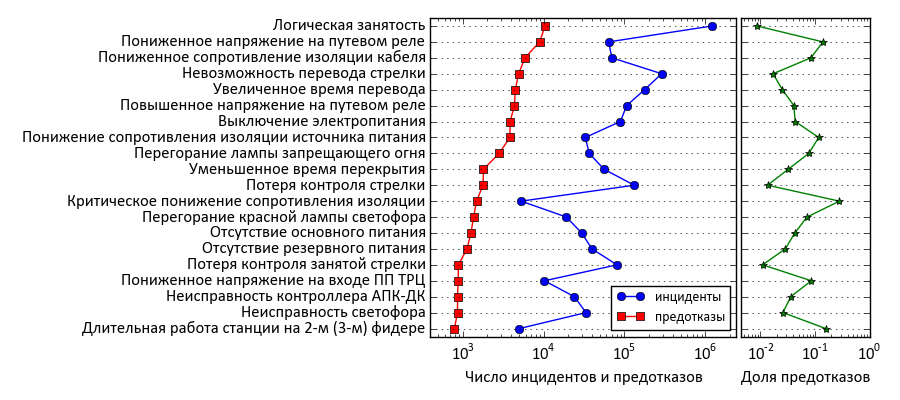
\includegraphics[width=10cm]{incidentsvsfaults-lines.png}
% 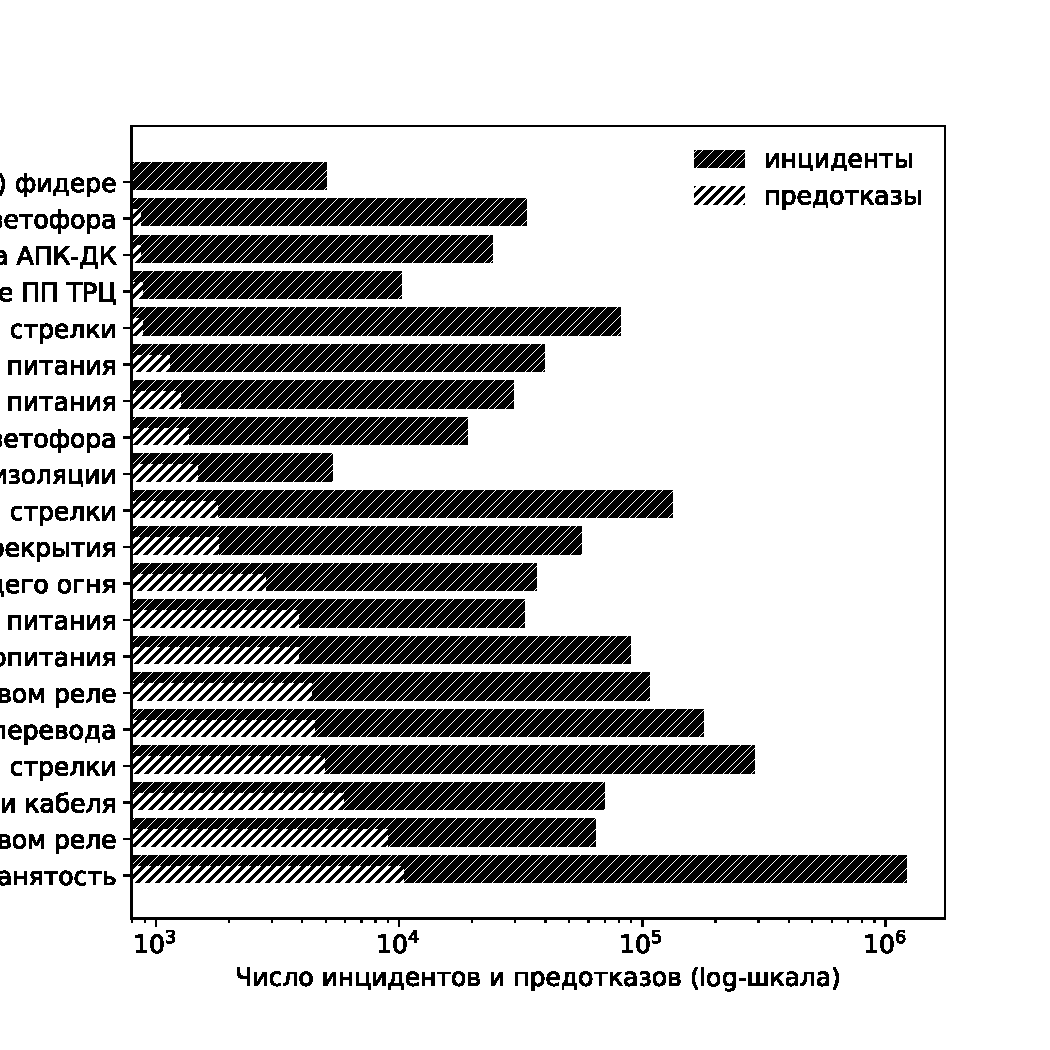
\includegraphics[width=14cm]{incidentsvsfaults-2}
\caption{Наиболее распространённые типы ситуаций, приводящих к предотказу}
\centering
\label{fig:histblue}
\end{figure*}

\begin{figure}[t]
\centering
% 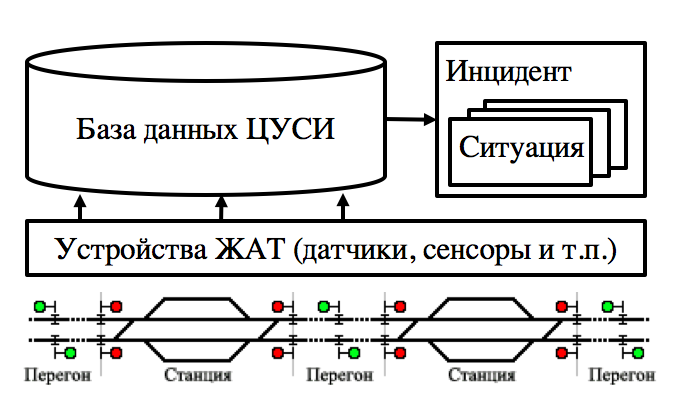
\includegraphics[width=10cm]{arch}


\tikzset{every picture/.style={line width=0.75pt}} %set default line width to 0.75pt

\begin{tikzpicture}[x=0.75pt,y=0.75pt,yscale=-1,xscale=1]
%uncomment if require: \path (0,236); %set diagram left start at 0, and has height of 236

\draw    (15.33, 119.33) rectangle (374.33, 149.33)   ;

\draw    (210.67, 9) rectangle (375, 79)   ;
\draw  [fill={rgb, 255:red, 255; green, 255; blue, 255 }  ,fill opacity=1 ]  (180.67, 18) rectangle (339.67, 88)   ;
\draw  [fill={rgb, 255:red, 255; green, 255; blue, 255 }  ,fill opacity=1 ]  (232.17, 40) rectangle (302.17, 73)   ;
\draw  [fill={rgb, 255:red, 255; green, 255; blue, 255 }  ,fill opacity=1 ]  (210.67, 44) rectangle (280.67, 77)   ;
\draw  [fill={rgb, 255:red, 255; green, 255; blue, 255 }  ,fill opacity=1 ]  (188.17, 48) rectangle (258.17, 81)   ;

\draw    (79.8, 23.64) circle [x radius= 65.2, y radius= 15.36]  ;
 \path   (144.95,71.99) .. controls (144.98,72.21) and (145,72.43) .. (145,72.65) .. controls (145,81.68) and (115.9,89) .. (80,89) .. controls (44.1,89) and (15,81.68) .. (15,72.65) -- (80, 72.64618359784444) -- cycle ;
 \draw   (144.95,71.99) .. controls (144.98,72.21) and (145,72.43) .. (145,72.65) .. controls (145,81.68) and (115.9,89) .. (80,89) .. controls (44.1,89) and (15,81.68) .. (15,72.65) ;
\draw    (14.59,23.15) -- (15,72.65) ;


\draw    (145,23.15) -- (144.95,71.99) ;



\draw [line width=1.5]    (55,119) -- (55,92) ;
\draw [shift={(55,89)}, rotate = 450] [fill={rgb, 255:red, 0; green, 0; blue, 0 }  ][line width=1.5]  [draw opacity=0] (11.61,-5.58) -- (0,0) -- (11.61,5.58) -- cycle    ;

\draw [line width=1.5]    (106,118.67) -- (106,91.67) ;
\draw [shift={(106,88.67)}, rotate = 450] [fill={rgb, 255:red, 0; green, 0; blue, 0 }  ][line width=1.5]  [draw opacity=0] (11.61,-5.58) -- (0,0) -- (11.61,5.58) -- cycle    ;

\draw [line width=1.5]    (81,119.33) -- (81,92.33) ;
\draw [shift={(81,89.33)}, rotate = 450] [fill={rgb, 255:red, 0; green, 0; blue, 0 }  ][line width=1.5]  [draw opacity=0] (11.61,-5.58) -- (0,0) -- (11.61,5.58) -- cycle    ;

\draw [line width=1.5]    (144.97,47.57) -- (177.22,47.57) ;
\draw [shift={(180.22,47.57)}, rotate = 540] [fill={rgb, 255:red, 0; green, 0; blue, 0 }  ][line width=1.5]  [draw opacity=0] (11.61,-5.58) -- (0,0) -- (11.61,5.58) -- cycle    ;

\draw    (16.67,172.95) -- (18.81,172.95) ;


\draw    (22.67,173) -- (46.67,173) ;


\draw    (34.67,170.33) -- (36.81,170.33) ;


\draw    (36.81,170.33) -- (36.81,176.36) ;


\draw    (34.67,176.36) -- (36.81,176.36) ;


\draw    (36.81,176.36) -- (38.96,176.36) ;


\draw    (36.81,170.33) -- (38.96,170.33) ;



\draw [line width=0.75]    (36.67,159.89) -- (36.81,167.22) ;


\draw [line width=0.75]    (30.63,163.56) -- (36.74,163.56) ;


\draw  [fill={rgb, 255:red, 0; green, 255; blue, 42 }  ,fill opacity=1 ][line width=0.75]   (28.3, 163.56) circle [x radius= 2.33, y radius= 2.26]  ;
\draw    (48.56,173) -- (50.88,173) ;


\draw    (52.08,173) -- (54.4,173) ;


\draw    (55.68,173) -- (58,173) ;


\draw    (59.76,173) -- (96.67,173) -- (109.77,159.9) -- (133.67,159.9) -- (145.22,173) -- (182.06,173) ;


\draw    (96.67,173) -- (145.22,173) ;


\draw    (68.22,170.11) -- (70.37,170.11) ;


\draw    (70.37,170.11) -- (70.37,176.14) ;


\draw    (68.22,176.14) -- (70.37,176.14) ;


\draw    (70.37,176.14) -- (72.52,176.14) ;


\draw    (70.37,170.11) -- (72.52,170.11) ;



\draw    (70,159.67) -- (70.15,167) ;


\draw    (70.07,163.33) -- (76.18,163.33) ;


\draw  [fill={rgb, 255:red, 255; green, 0; blue, 0 }  ,fill opacity=1 ]  (78.63, 163.53) circle [x radius= 2.33, y radius= 2.26]  ;
\draw    (170.67,170.11) -- (172.81,170.11) ;


\draw    (172.81,170.11) -- (172.81,176.14) ;


\draw    (170.67,176.14) -- (172.81,176.14) ;


\draw    (172.81,176.14) -- (174.96,176.14) ;


\draw    (172.81,170.11) -- (174.96,170.11) ;



\draw [line width=0.75]    (172.67,159.22) -- (172.81,166.56) ;


\draw [line width=0.75]    (166.63,162.89) -- (172.74,162.89) ;


\draw  [fill={rgb, 255:red, 255; green, 26; blue, 0 }  ,fill opacity=1 ][line width=0.75]   (164.3, 162.89) circle [x radius= 2.33, y radius= 2.26]  ;
\draw    (16.95,186.38) -- (19.1,186.38) ;


\draw    (22.95,186.43) -- (46.95,186.43) ;


\draw    (34.95,183.76) -- (37.1,183.76) ;


\draw    (37.1,183.76) -- (37.1,189.79) ;


\draw    (34.95,189.79) -- (37.1,189.79) ;


\draw    (37.1,189.79) -- (39.25,189.79) ;


\draw    (37.1,183.76) -- (39.25,183.76) ;



\draw    (48.85,186.43) -- (51.17,186.43) ;


\draw    (52.37,186.43) -- (54.69,186.43) ;


\draw    (55.97,186.43) -- (58.29,186.43) ;


\draw    (60.05,186.43) -- (96.95,186.43) -- (110.53,200) -- (134.51,200) -- (145.5,186.43) -- (182.35,186.43) ;


\draw    (96.95,186.43) -- (145.5,186.43) ;


\draw    (68.51,183.54) -- (70.66,183.54) ;


\draw    (70.66,183.54) -- (70.66,189.57) ;


\draw    (68.51,189.57) -- (70.66,189.57) ;


\draw    (70.66,189.57) -- (72.8,189.57) ;


\draw    (70.66,183.54) -- (72.8,183.54) ;



\draw    (70.51,192.65) -- (70.66,199.98) ;


\draw    (70.58,196.32) -- (76.69,196.32) ;


\draw  [fill={rgb, 255:red, 255; green, 0; blue, 0 }  ,fill opacity=1 ]  (79.14, 196.52) circle [x radius= 2.33, y radius= 2.26]  ;
\draw    (170.95,183.54) -- (173.1,183.54) ;


\draw    (173.1,183.54) -- (173.1,189.57) ;


\draw    (170.95,189.57) -- (173.1,189.57) ;


\draw    (173.1,189.57) -- (175.25,189.57) ;


\draw    (173.1,183.54) -- (175.25,183.54) ;



\draw [line width=0.75]    (173.2,192.4) -- (173.35,199.73) ;


\draw [line width=0.75]    (167.17,196.07) -- (173.28,196.07) ;


\draw  [fill={rgb, 255:red, 255; green, 26; blue, 0 }  ,fill opacity=1 ][line width=0.75]   (164.84, 196.07) circle [x radius= 2.33, y radius= 2.26]  ;
\draw    (36.89,193.03) -- (37.04,200.37) ;


\draw    (36.96,196.7) -- (43.07,196.7) ;


\draw  [fill={rgb, 255:red, 0; green, 255; blue, 16 }  ,fill opacity=1 ]  (45.52, 196.9) circle [x radius= 2.33, y radius= 2.26]  ;
\draw    (91.8,173.13) -- (78.5,186.43) ;


\draw    (163.64,173) -- (150.34,186.3) ;



\draw    (176,173.28) -- (178.15,173.28) ;


\draw    (182,173.33) -- (206,173.33) ;


\draw    (194,170.67) -- (196.15,170.67) ;


\draw    (196.15,170.67) -- (196.15,176.69) ;


\draw    (194,176.69) -- (196.15,176.69) ;


\draw    (196.15,176.69) -- (198.3,176.69) ;


\draw    (196.15,170.67) -- (198.3,170.67) ;



\draw [line width=0.75]    (196,160.22) -- (196.15,167.56) ;


\draw [line width=0.75]    (189.97,163.89) -- (196.07,163.89) ;


\draw  [fill={rgb, 255:red, 0; green, 255; blue, 42 }  ,fill opacity=1 ][line width=0.75]   (187.63, 163.89) circle [x radius= 2.33, y radius= 2.26]  ;
\draw    (207.9,173.33) -- (210.22,173.33) ;


\draw    (211.42,173.33) -- (213.73,173.33) ;


\draw    (215.02,173.33) -- (217.33,173.33) ;


\draw    (219.1,173.33) -- (256,173.33) -- (269.1,160.23) -- (293,160.23) -- (304.55,173.33) -- (341.4,173.33) ;


\draw    (256,173.33) -- (304.55,173.33) ;


\draw    (227.56,170.44) -- (229.7,170.44) ;


\draw    (229.7,170.44) -- (229.7,176.47) ;


\draw    (227.56,176.47) -- (229.7,176.47) ;


\draw    (229.7,176.47) -- (231.85,176.47) ;


\draw    (229.7,170.44) -- (231.85,170.44) ;



\draw    (229.33,160) -- (229.48,167.33) ;


\draw    (229.41,163.67) -- (235.51,163.67) ;


\draw  [fill={rgb, 255:red, 255; green, 0; blue, 0 }  ,fill opacity=1 ]  (237.97, 163.87) circle [x radius= 2.33, y radius= 2.26]  ;
\draw    (330,170.44) -- (332.15,170.44) ;


\draw    (332.15,170.44) -- (332.15,176.47) ;


\draw    (330,176.47) -- (332.15,176.47) ;


\draw    (332.15,176.47) -- (334.3,176.47) ;


\draw    (332.15,170.44) -- (334.3,170.44) ;



\draw [line width=0.75]    (332,159.56) -- (332.15,166.89) ;


\draw [line width=0.75]    (325.97,163.22) -- (332.07,163.22) ;


\draw  [fill={rgb, 255:red, 255; green, 26; blue, 0 }  ,fill opacity=1 ][line width=0.75]   (323.63, 163.22) circle [x radius= 2.33, y radius= 2.26]  ;
\draw    (176.29,186.71) -- (178.43,186.71) ;


\draw    (182.29,186.76) -- (206.29,186.76) ;


\draw    (194.29,184.1) -- (196.43,184.1) ;


\draw    (196.43,184.1) -- (196.43,190.12) ;


\draw    (194.29,190.12) -- (196.43,190.12) ;


\draw    (196.43,190.12) -- (198.58,190.12) ;


\draw    (196.43,184.1) -- (198.58,184.1) ;



\draw    (208.18,186.76) -- (210.5,186.76) ;


\draw    (211.7,186.76) -- (214.02,186.76) ;


\draw    (215.3,186.76) -- (217.62,186.76) ;


\draw    (219.38,186.76) -- (256.29,186.76) -- (269.86,200.34) -- (293.84,200.34) -- (304.84,186.76) -- (341.68,186.76) ;


\draw    (256.29,186.76) -- (304.84,186.76) ;


\draw    (227.84,183.87) -- (229.99,183.87) ;


\draw    (229.99,183.87) -- (229.99,189.9) ;


\draw    (227.84,189.9) -- (229.99,189.9) ;


\draw    (229.99,189.9) -- (232.14,189.9) ;


\draw    (229.99,183.87) -- (232.14,183.87) ;



\draw    (229.84,192.98) -- (229.99,200.32) ;


\draw    (229.92,196.65) -- (236.02,196.65) ;


\draw  [fill={rgb, 255:red, 255; green, 0; blue, 0 }  ,fill opacity=1 ]  (238.47, 196.85) circle [x radius= 2.33, y radius= 2.26]  ;
\draw    (330.29,183.87) -- (332.43,183.87) ;


\draw    (332.43,183.87) -- (332.43,189.9) ;


\draw    (330.29,189.9) -- (332.43,189.9) ;


\draw    (332.43,189.9) -- (334.58,189.9) ;


\draw    (332.43,183.87) -- (334.58,183.87) ;



\draw [line width=0.75]    (332.54,192.73) -- (332.68,200.07) ;


\draw [line width=0.75]    (326.5,196.4) -- (332.61,196.4) ;


\draw  [fill={rgb, 255:red, 255; green, 26; blue, 0 }  ,fill opacity=1 ][line width=0.75]   (324.17, 196.4) circle [x radius= 2.33, y radius= 2.26]  ;
\draw    (196.22,193.37) -- (196.37,200.7) ;


\draw    (196.3,197.03) -- (202.4,197.03) ;


\draw  [fill={rgb, 255:red, 0; green, 255; blue, 16 }  ,fill opacity=1 ]  (204.86, 197.23) circle [x radius= 2.33, y radius= 2.26]  ;
\draw    (251.13,173.46) -- (237.83,186.76) ;


\draw    (322.97,173.33) -- (309.67,186.63) ;



\draw    (335.67,173.28) -- (337.81,173.28) ;


\draw    (341.67,173.33) -- (365.67,173.33) ;


\draw    (353.67,170.67) -- (355.81,170.67) ;


\draw    (355.81,170.67) -- (355.81,176.69) ;


\draw    (353.67,176.69) -- (355.81,176.69) ;


\draw    (355.81,176.69) -- (357.96,176.69) ;


\draw    (355.81,170.67) -- (357.96,170.67) ;



\draw [line width=0.75]    (355.67,160.22) -- (355.81,167.56) ;


\draw [line width=0.75]    (349.63,163.89) -- (355.74,163.89) ;


\draw  [fill={rgb, 255:red, 0; green, 255; blue, 42 }  ,fill opacity=1 ][line width=0.75]   (347.3, 163.89) circle [x radius= 2.33, y radius= 2.26]  ;
\draw    (367.56,173.33) -- (369.88,173.33) ;


\draw    (371.08,173.33) -- (373.4,173.33) ;


\draw    (374.68,173.33) -- (377,173.33) ;


\draw    (335.95,186.71) -- (338.1,186.71) ;


\draw    (341.95,186.76) -- (365.95,186.76) ;


\draw    (353.95,184.1) -- (356.1,184.1) ;


\draw    (356.1,184.1) -- (356.1,190.12) ;


\draw    (353.95,190.12) -- (356.1,190.12) ;


\draw    (356.1,190.12) -- (358.25,190.12) ;


\draw    (356.1,184.1) -- (358.25,184.1) ;



\draw    (367.85,186.76) -- (370.17,186.76) ;


\draw    (371.37,186.76) -- (373.69,186.76) ;


\draw    (374.97,186.76) -- (377.29,186.76) ;


\draw    (355.89,193.37) -- (356.04,200.7) ;


\draw    (355.96,197.03) -- (362.07,197.03) ;


\draw  [fill={rgb, 255:red, 0; green, 255; blue, 16 }  ,fill opacity=1 ]  (364.52, 197.23) circle [x radius= 2.33, y radius= 2.26]  ;


\draw (80,59) node [scale=1] [align=left] {БД ЦУСИ};
\draw (194.33,133.33) node [scale=1] [align=left] {Устройства ЖАТ (датчики, сенсоры и т.п.)};
\draw (220,31) node [scale=1] [align=left] {Инцидент};
\draw (223,64.5) node [scale=1] [align=left] {Ситуация};
\draw (126.67,213) node [scale=1] [align=left] {Станция};
\draw (46.67,213) node [scale=1] [align=left] {Перегон};
\draw (286,213.33) node [scale=1] [align=left] {Станция};
\draw (206,213.33) node [scale=1] [align=left] {Перегон};


\end{tikzpicture}

\caption{Последовательность формирования инцидентов: архитектура системы мониторинга}
\centering
\label{fig:arch}
\end{figure}
\textbf{Задача} состоит в том, чтобы автоматически классифицировать инциденты, регистрируемые устройствами железнодорожной автоматики и телемеханики,  по их признакам на неисправности, ТОиР и т.п. В качестве \textbf{входных данных} могут использоваться все известные на текущий момент параметры инцидента (признаки места, времени, типа события, показания датчиков и т.п.) и его контекст (например, погода, прошлые инциденты и т.п.). \textbf{Выходные данные}: вероятность того, что инцидент связан с предотказом контролируемого объекта (число от 0 до 1).
Отметим, что важность инцидента можно считать определяемой двумя факторами: вероятностью того, что данный инцидент является реальным предотказным состоянием, и последствиями (в частности, экономическим эффектом) данного отказа. Эти два фактора имеют совершенно разный характер и в значительной степени независимы друг от друга. В то время как вероятность предотказного состояния является предметом статистического анализа на основе лишь сохраненных оперативных данных об инцидентах, оценка последствий отказа предполагает привлечение дополнительных стоимостных моделей отказов и других соображений. В настоящей работе мы акцентируем внимание лишь на первом, вероятностном факторе важности; второй фактор учитывается ЦУСИ МЖД отдельно, с помощью нескольких альтернативных моделей.
С учетом сделанного замечания цель данной работы можно сформулировать как построение прогнозной модели, которая предсказывает вероятность предотказного состояния для данного инцидента на основе автоматически сформированных данных об этом инциденте.
Каждый инцидент в базе данных ЦУСИ представляет собой набор ситуаций -- единичных событий, несущих признаки предотказного состояния (например, повышение напряжения, понижение сопротивления и т.п.), см. рис. \ref{fig:arch}. Ситуации автоматически объединяются в инциденты на этапе предварительной обработки сигналов датчиков. В простейшем случае инцидент содержит несколько последовательных однотипных ситуаций (например, несколько случаев кратковременного повышения напряжения на одном и том же приборе), но может содержать и разнотипные ситуации, затрагивающие разное оборудование (например, увеличенное время перевода стрелки и некорректные параметры тока перевода). Количество ситуаций в инциденте может варьироваться от одного до нескольких сотен и может увеличиваться со временем, пока инцидент не рассмотрен и не закрыт оператором ЦУСИ. В общей сложности база данных ЦУСИ содержит около 5 млн. инцидентов, включающих 100 млн. ситуаций.

Описание каждой ситуации содержит ее тип, время начала и окончания,
ID места (станции или перегона), ID объекта измерения (прибора) и некоторые другие, менее существенные элементы. Большинство свойств (кроме времени) являются категориальными, причем количество их значений может быть достаточно большим: данные охватывают несколько сот типов ситуаций и мест и около 65000 приборов.

При закрытии инцидента оператором ставится пометка о выявленном типе инцидента, в частности являлся ли он предотказом.

Таким образом, исторические данные содержат достаточно богатую и хорошо структурированную информацию для построения сложных прогностических моделей вероятности предотказа.
В качестве примера простой предсказательной модели можно привести прогноз вероятности предотказного состояния исключительно на основе типа первой ситуации инцидента, а именно как долю предотказных инцидентов среди всех наблюдавшихся ранее инцидентов с первой ситуацией данного типа. Это доля сильно зависит от типа ситуации, например, из рис. \ref{fig:histblue} видно, что для ситуации «Критическое понижение сопротивления изоляции» она значительно выше, чем для «Потери контроля занятой стрелки». Поскольку различных типов ситуаций несколько сотен и операторы, очевидно, не в состоянии помнить характеристики каждой из них, даже эта простейшая автоматическая модель ранжирования оказывается практически полезной. В дальнейшем мы будем называть эту модель ``референсной''.
Машинное обучение (МО) Машинное обучение на основе имеющихся исторических данных об инцидентах позволяет строить гораздо более точные предсказательные модели. Стандартная практика машинного обучения \cite{hastie01statisticallearning, Mitchell:1997:ML:541177, scikit-learn} предполагает построение модели в два этапа:
\begin{enumerate}
\item извлечение признаков и формирование обучающей матрицы;
\item применение к полученной обучающей матрице некоторого общего МО-алгоритма.
\end{enumerate}
В ходе первого этапа информация о каждом инциденте приводится к унифицированному виду числового вектора фиксированной размерности, компоненты которого (признаки) отражают потенциально существенные для прогноза характеристики инцидента.
В ходе второго этапа к полученной обучающей матрице обычно применяется один из стандартных МО-алгоритмов: логистическая регрессия, нейронные сети, ансамбли решающих деревьев и т.п. Нами использовался алгоритм XGBoost построения ансамбля решающих деревьев с помощью градиентного бустинга \cite{chen2016xgboost}.
Извлечение признаков являлось наиболее творческой и трудоемкой частью решения задачи. Оно было связано со следующими трудностями:
\begin{itemize}
\item В общем случае, признаки необходимо агрегировать из всех ситуаций данного инцидента, учитывая, что ситуаций может быть произвольное число. Нами были рассмотрены различные стратегии агрегации, например: ограничиться первой или последней ситуацией в инциденте; в случае числовых признаков взять максимум, минимум или среднее значение по всем ситуациям; в случае категориальных признаков отметить все категории, встреченные в ситуациях инцидентах или сосчитать количество различных встреченных категорий. Конечно, некоторые признаки естественным образом связаны с инцидентом в целом (например, полная продолжительность или место инцидента).
\item Естественным способом преобразования категориального признака с $N$ возможными значениями в числовую форму является его кодирование в виде вектора длины $N$ с единственным ненулевым элементом (one-hot-encoding). Ввиду того, что в рассматриваемой задаче $N$ достигает нескольких сотен или даже тысяч,  обучающие матрицы реализовывались нами в виде разреженных матриц.
\end{itemize}
С учетом этих обстоятельств, мы рассмотрели несколько десятков различных признаков, описывающих пространственно-временные и прочие характеристики инцидентов.

Важную роль при создании и отборе признаков играла оценка их значимости, которая осуществлялась нами с помощью двух методов.
\begin{itemize}
\item
Во-первых, мы оценивали важность признака по общему числу соответствующих ветвлений в итоговой предсказательной модели -- лесе решающих деревьев. Для ``сильно ветвящихся'' признаков мы производили попытку самостоятельно разбить признак на несколько вспомогательных.
\item Во-вторых, мы реализовали жадный переборный алгоритм последовательного добавления в модель новых признаков, дающих наибольших прирост точности. Этот способ требует многократного обучения модели на различных наборах признаков и поэтому сравнительно долог, однако он позволяет понять, несут ли новые признаки какую-то существенную новую информацию по отношению к уже имеющимся, и какой минимальный набор признаков обеспечивает приемлемую точность модели.
\end{itemize}
Отметим, что помимо признаков, извлекаемых из базы инцидентов, нами была сделана попытка сформировать дополнительные признаки на основе метеоданных, поскольку погодные условия, очевидно, должны оказывать сильное влияние на возникновение некоторых предотказных состояний. Мы действительно обнаружили наличие корреляций между погодными признаками и количеством инцидентов, однако добавление этих признаков в нашу модель не дало заметного улучшения. Иными словами, информация о погоде позволяет улучшить прогноз возникновения инцидента при отсутствии иной информации, но не позволяет заметно улучшить прогноз предотказа при наличии уже имеющейся в базе данных информации об инциденте.


Отметим следующие наблюдения:
\begin{itemize}
\item Как обсуждается далее, включение в обучающую выборку признаков, родственных уже имеющимся, не дает прироста точности прогноза.
При этом оказалось довольно эффективным сформировать несколько различных признаков, зависящих лишь от времени (полная продолжительность инцидента, время суток и день недели, максимальная продолжительность ситуаций и др.).
\item Погодные условия, очевидно, должны оказывать сильное влияние на возникновение некоторых инцидентов. Нами была сделана попытка привлечь метеоданные для улучшения точности предсказательной модели, однако добавление соответствующих признаков не привело к заметному улучшению. С другой стороны, мы действительно наблюдали наличие корреляций между погодными признаками и количеством инцидентов. Иными словами, информация о погоде позволяет улучшить прогноз возникновения инцидента при отсутствии иной информации, но не позволяет заметно улучшить прогноз предотказа при наличии уже имеющейся в базе данных информации об инциденте.
\end{itemize}
Предсказательная модель строилась нами с помощью библиотеки XGboost \cite{chen2016xgboost}. Эта открытая библиотека, хорошо зарекомендовавшая себя в большом числе задач анализа данных\cite{chen2016xgboost}. За последнее время XGBoost неоднократно использовался для решения индустриальных задач, таких как предсказание потребления топлива \cite{horituchi2017predicting}, сбоев технологических процессов (\cite{bosch,DBLP:conf/bigdataconf/Hebert16}), и различных свойств химических составов(\cite{sheridan2016extreme,babajide2016bioactive}). XGboost содержит эффективную реализацию градиентного бустинга \cite{friedman2001greedy}, поддерживающую большие выборки и разреженные матрицы, что было важно в данном проекте. Предсказательная модель представляется в виде суммы ансамбля  бинарных решающих деревьев, последовательно добавляемых в ходе обучения.

Заметим, что референсная модель также естественным образом реализуется в виде ансамбля решающих деревьев, построенных по одному категориальному признаку -- типу первого инцидента. А именно, она состоит из тривиальных деревьев глубины 1 (``решающих пней''), по одному на каждую из компонент бинарного вектора, кодирующего этот категориальный признак. Таким образом, наша основная модель является естественным обобщением референсной модели на случай произвольного набора признаков, числа деревьев и их глубины.

Основная модель была обучена по 3 годам исторических данных (около 5.3 млн. инцидентов) и включала в себя 4000 деревьев глубины 10. Подбор параметров модели осуществлялся стандартным образом с помощью тестирования на контрольной части обучающей выборки.
Современные методы машинного обучения позволяют, добиться гораздо большей точности прогноза путем учета большого числа признаков предотказного состояния в рамках сложной логической структуры, массива всех исторических наблюдений. В рамках предложенного подхода была предложена следующая стратегия порождения решающего правила.
Ниже описывается процедура предварительной обработки исходных данных, содержащихся в базе инцидентов.
\begin{itemize}
\item Исправление пропусков и некорректных значений. На этом этапе для каждого признака порождается дополнительный признак – индикатор некорректного значения. Для численных признаков значение заменяется средним значением, для категориальных – индикатором пропуска.
\item Нормализация распределений численных переменных. На этом этапе подбирается трансформация, преобразующая множество значений величины в отрезок [0;1].
\item Текстовые и категориальные признаки бинаризуются, категориальный признак с множеством значений размера N заменяется разреженной матрицей с N+1 столбцами. На практике встречающиеся редко величины признаков принято объединять в один признак. В данной работе такой подход не использовался. Вместо этого производился анализ значимости каждого признака с последующим выбором наиболее важных.
\end{itemize}

Параметры соответствующих преобразований над множеством признаков сохраняются индивидуально для каждого признака. Эти преобразования далее применяются повторно при обработке инцидентов в реальном времени.
Самый трудоемкий этап подготовки массива данных – порождение сложных признаков из множества простых, хранящихся в базе данных. При порождении такого рода признаков требуется следить за тем, что аналогичные признаки могли бы быть посчитаны не только по историческому массиву данных, но и в оперативном режиме работы классификатора.

\begin{itemize}
\item Из исходного признака времени порождаются признаки выходных и праздничных дней, времени суток. В качестве независимых признаков выделяются также номера дня в году, месяце и неделе, номер месяца, час, минута и секунда начала инцидента.
\item Признаки времени и места также дополнялись признаками погодных условий – давление, температура, влажность и скорость ветра.
\item Признаки территориальной принадлежности (номер дистанции, номер объекта) дополняются кластеризующими признаками. В нашем случае для кластеризации удалось воспользоваться номером объекта в базе данных (объекты в базе нумеруются последовательно с внедрением и неявно несут информацию о времени и месте установки).
\item Признаки, характеризующие частоту поступления инцидентов для того или иного типа объекта ЖАТ (стрелки, светофоры, рельсовые цепи) для разных временных промежутков (от 1 минуты до месяца). Аналогичные составные признаки были выделены для различных мест обнаружения инцидентов (станция, перегон и т.д.).
\end{itemize}
Заключительный этап подготовки данных заключается в проверке статистической значимости переменных в модели. Этот шаг выполняется, чтобы отбросить шумящие переменные. Для оценки значимости признаков в данной работе использовалось два подхода.

Первый подход заключается в исследовании поведения показателя AUC при добавлении нового признака на вход обучаемого классификатора. В этом случае для ускорения расчетов мы используем заниженное значение количества раундов обучения и жадный алгоритм выбора очередного признака. Более важным признаком будем считать такой признак, при добавлении которого достигается максимальное увеличение площади под операционной характеристикой классификатора. Эффективность каждого отдельного признака показана на \ref{fig:initialFeatureScores}. На рисунке \ref{fig:adaptiveAdditionScores} можно увидеть последовательное изменение величины показателя AUC при добавлении новых признаков. На рисунке \ref{fig:adaptiveAdditionScores} показано насколько больший прирост дает добавляемый признак по сравнению с еще не добавленными.

Второй подход заключается в изучении количественных характеристик итогового решающего правила (леса решающих деревьев) на всем множестве признаков после прохода раундов обучения. В этом случае более важным признаком будем считать такой признак, которому соответствует большее суммарное количество разветвлений в итоговом решающем правиле. Для "сильно ветвящийся" признаков мы производили попытку самостоятельно разбить признак на несколько вспомогательных.

\begin{figure*}
\centering
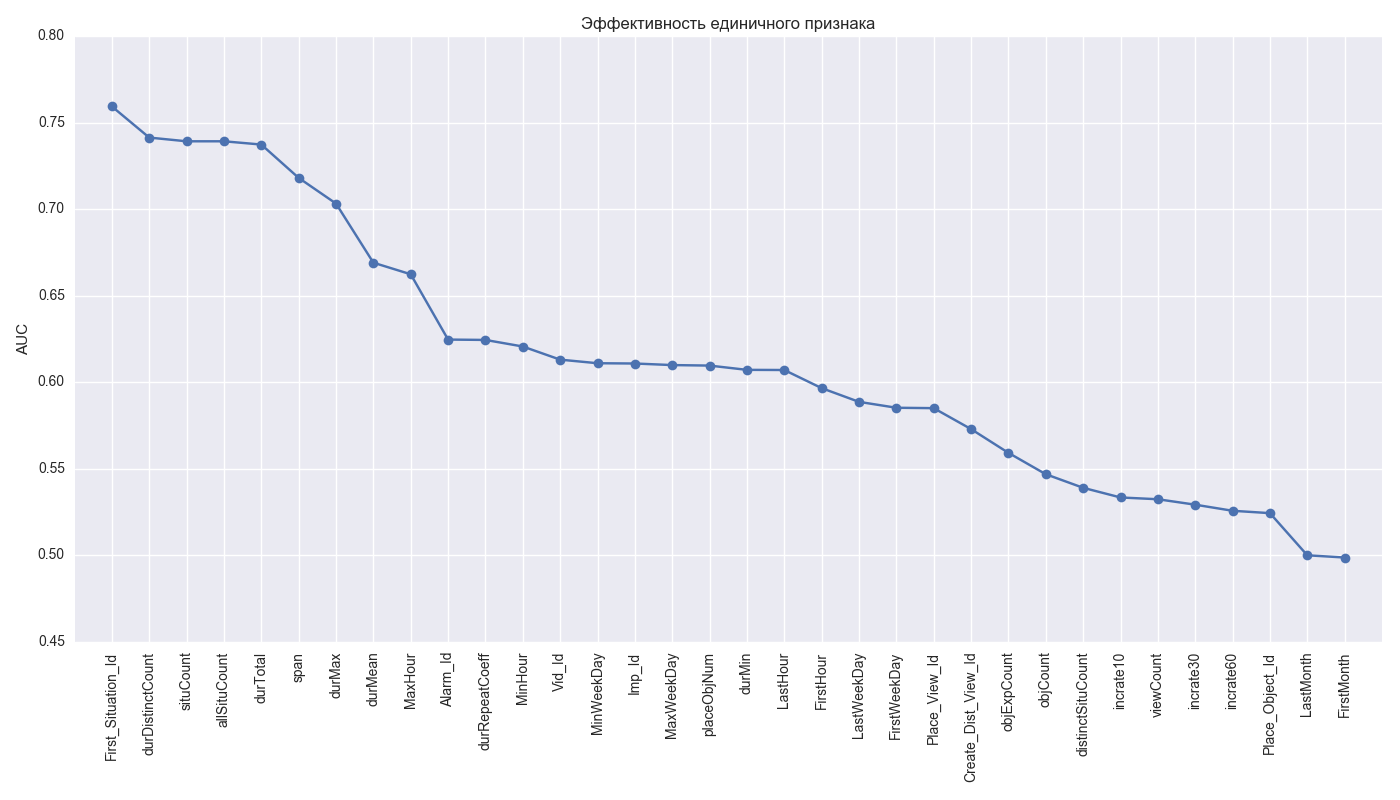
\includegraphics[width=10cm]{initialFeatureScores}
\caption{Анализ важности признаков: эффективность отдельных признаков}
\centering
\label{fig:initialFeatureScores}
\end{figure*}

Построенная нами высокоточная прогнозная модель имеет вид ансамбля глубоких решающих деревьев \cite{friedman2001greedy}
включает в себя 4000 деревьев глубины 10.

Окончательный прогноз вероятности предотказа получается усреднением прогнозов по всем деревьям.


%\pagecolor{yellow!30!orange}
\begin{figure}[thpb]
\centering
% \includegraphics[width=7cm]{histo2}
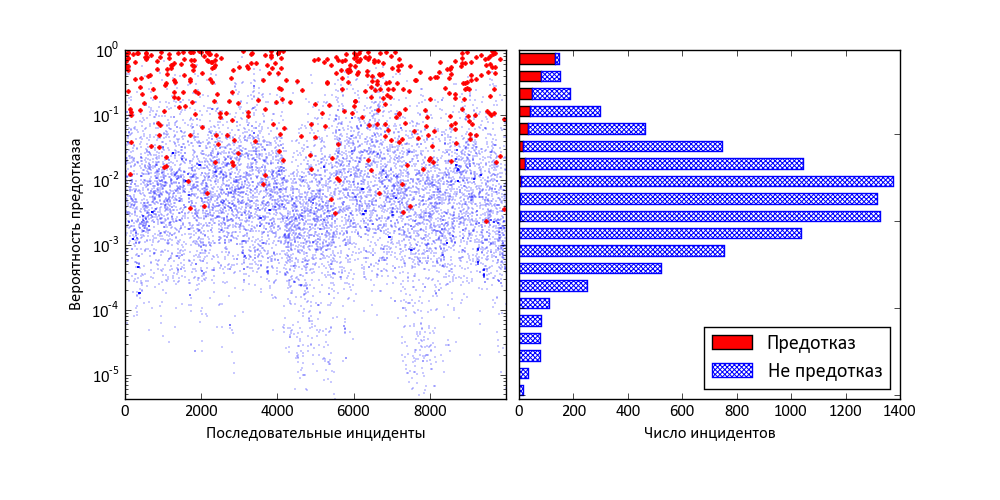
\includegraphics[trim=7mm 7mm 11mm 5mm, clip, width=\textwidth]{threswall-plus.png}
\caption{Результаты ранжирования 10000 последовательных инцидентов.  Предотказы показаны крупными точками, ложные тревоги -- мелкими. В правой части рисунка показаны соответствующие гистограммы распределения инцидентов по вероятности.}
\centering
\label{fig:histo}
\end{figure}

В соответствии со стандартной практикой машинного обучения, тестирование построенной модели проводилось на тестовой выборке, изолированной от обучающей выборки, причем обучающие инциденты предшествовали по времени тестовым.

На рисунке \ref{fig:histo} приведены результаты ранжирования 10000 последовательных инцидентов. Крупные точки показывают инциденты, связанные с предотказами, а мелкие -- инциденты, связанные с ложными срабатываниями системы. Хорошо видно, что основная масса предотказов имеет высокую вероятность и визуально отделена по вероятности от основной массы ложных тревог, имеющей меньшую вероятность. Это свидетельствует о пригодности использования предсказательной модели в качестве ранжирующей функции.

Из рисунка очевидна некоторая неравномерность и периодичность распределения вероятности предотказа в зависимости от номера инцидента. Этот эффект объясняется суточным циклом (показанные 10000 инцидентов отвечают временному интервалу продолжительностью около 3 дней). В дневное время значительное число инцидентов связано с техническим обслуживанием и ремонтом; модель присваивает низкую вероятность предотказа таким инцидентам.


Следует отметить, что существенная доля предотказов имеет после классификации значение вероятности в промежутке 0.001 и 0.1. Для удобства восприятия, это значение выводится на экран инженера службы мониторинга в логарифмической шкале. На рисунке 6 представлена гистограмма распределения значения ранга после логарифмического преобразования. Видно, что большинство инцидентов, связанных с предотказами, находится в промежутке 0.5 – 1.0.

Для количественной оценки эффективности ранжирования мы используем кривую ошибок, определяемую следующим образом. Предположим, что операторы успевают обрабатывать лишь некоторую долю всех инцидентов; рассмотрим соответствующую переменную ДОИ (Доля Обработанных Инцидентов) со значениями в интервале $[0,1]$. Будем считать, что операторы в первую очередь обрабатывают те инциденты, для которых модель предсказывает наиболее высокую вероятность отказа. Пусть величина ДОО (Доля Охваченных Отказов), также со значениями в интервале $[0,1]$, обозначает долю обрабатываемых при этом предотказных инцидентов среди всех предотказных инцидентов. Кривая ошибок тогда представляет собой график зависимости ДОО от ДОИ.

\begin{figure}[thb]
\centering
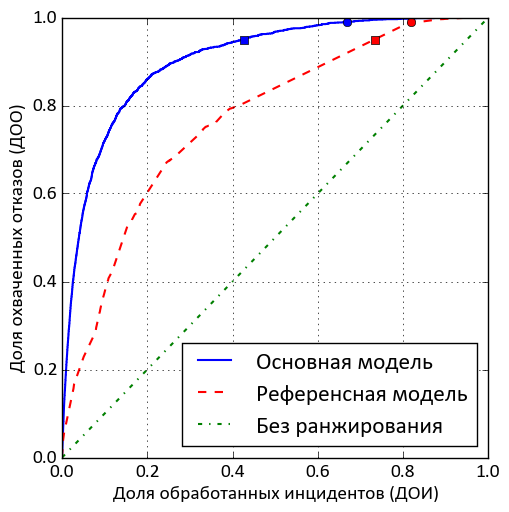
\includegraphics[width=0.5\textwidth]{latexRoc.png}
\caption{Кривые ошибок и связанные с ними характеристики для основной и референсной моделей. Выделенные точки отвечают ДОО 0.95 и  0.99.}\label{fig:ROCcurves}
\end{figure}

\begin{table} [htbp]
  \label{tbl:aucresults}
  \centering
  %\captionsetup{width=15cm}
  \caption{Количественные результаты ранжирования}\label{Ts0Sib}%
\begin{tabular}{ l c c c}
\toprule
Модель & AUC & ДОИ95 & ДОИ99 \\ \midrule
Основная & 0.904& 0.427 & 0.669 \\
Референсная & 0.768 & 0.733 & 0.818\\
\bottomrule
\end{tabular}
\end{table}

На рис. \ref{fig:ROCcurves} показаны кривые ошибок для основной и референсной моделей ранжирования. Чем выше лежит кривая, тем лучше. Максимально возможное положение кривой соответствует линейной функции $\text{ДОО}=\frac{ДОИ}{\alpha},$ где $\alpha\approx 0.024$ -- доля предотказов среди всех инцидентов. Если оператор выбирает инцидент наугад (без рассмотрения ранга), то кривая ошибок является диагональю квадрата.

В качестве основной количественной характеристики точности мы рассматриваем AUC (Area Under Curve) -- площадь под кривой ошибок. Ее значения для обеих моделей приведены в таблице на рис. \ref{fig:ROCcurves}. Кроме того, мы приводим значения ДОИ95\% и ДОИ99\%, которые определяются как те значение ДОИ, при которых ДОО составляет, соответственно, 0.95 и 0.99. Заметим, в частности, что если операторы обрабатывают лишь половину инцидентов, а именно те, которые имеют основной ранг выше медианного значения, то при этом пропускается менее 5\% предотказных состояний.


\begin{figure}[thpb]
\caption{Динамика точности ранжирования и ее прироста.}
\label{fig:adaptiveAdditionScores}
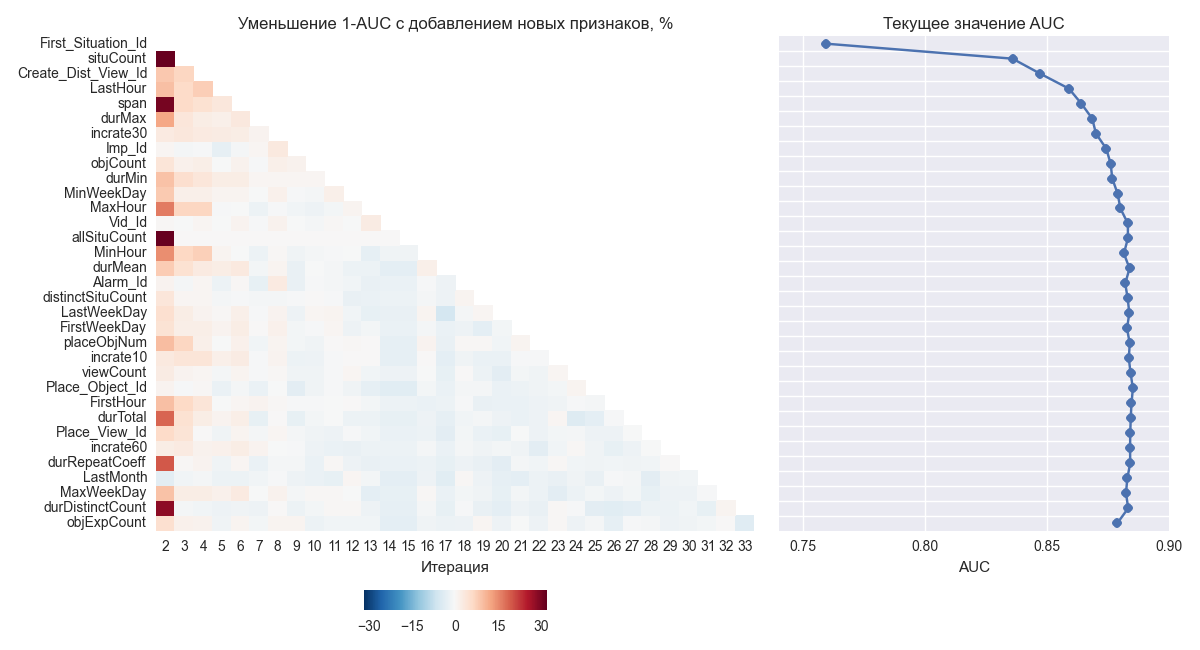
\includegraphics[width=\textwidth]{fullAdaptiveData.png}
\end{figure}


\todo{Анализ важности признаков с помощью их последовательного жадного добавления: на каждой итерации к текущему набору признаков, начиная с {\texttt First\_Situation\_id}, добавляется новый признак, при котором точность ранжирования увеличивается сильнее всего. Рис.~\ref{fig:adaptiveAdditionScores}  На диаграмме слева показаны относительные изменения величины $1-\textrm{AUC}$ при добавлении каждого из признаков, не входящих в текущий набор. График справа показывает динамику точности предсказательной модели, построенной по текущему набору признаков. Таблица~\ref{tbl:adaptiveAdditionScores} Несколько первых признаков, до насыщения модели.}

На рис. \ref{fig:adaptiveAdditionScores} показаны результаты эксперимента по последовательному адаптивному добавлению в модель новых признаков. На каждом шаге для каждого из еще не входящих в модель признаков совершается пересчет точности модели с этим дополнительным признаком; тот, для которого наблюдается наибольшее приращение точности, включается в модель. В общей сложности рассматривается 34 признака, процедура начинается с признака типа первой ситуации (как наиболее информативного).

В левой части рисунка \ref{fig:adaptiveAdditionScores}(a) показаны относительные изменения характеризующей ошибку величины $1-\text{AUC}$ для каждой итерации (горизонтальная ось) и каждого признака--кандидата (вертикальная ось). Признаки упорядочены post factum по очередности включения в модель, так что диаграмма имеет треугольный вид. В правой части рисунка показаны значения AUC соответствующей модели для каждой итерации. Для ускорения процедуры, модели в этом эксперименте строились с уменьшенным числом деревьев, поэтому их значения AUC ниже значения, указанного для основной модели на рис. \ref{fig:ROCcurves}.

В результате данного эксперимента мы видим, что модель насыщается после включения в нее 10 -- 15 признаков, и ее точность перестает существенно меняться, если не считать небольшого эффекта переобучения, наблюдаемого в конце эксперимента. Первые несколько признаков являются одновременно достаточно информативными и разнообразными; их описания приведены в таблице \ref{fig:adaptiveAdditionScores}(b). На левой части рис. \ref{fig:adaptiveAdditionScores}(a) хорошо видно, что полезность признаков падает с итерациями, причем падение является резким в моменты, когда в набор включается признак, родственный рассматриваемому (см., например, \texttt{span} и \texttt{situCount}). Несмотря на это, мы видим, что полезно иметь, например, много разных признаков, характеризующих время ситуаций.

\begin{figure}[thb]
\centering
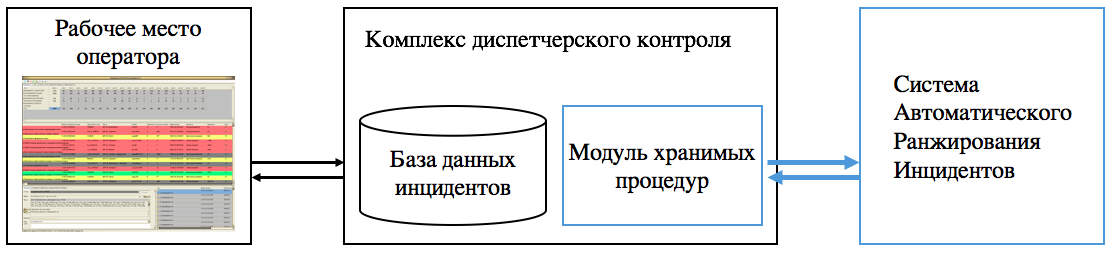
\includegraphics[width=10cm]{modules-v2}
\centering
\caption{Схема интеграции САРИ и АПК ДК.}
\centering
\label{fig:modules}
\end{figure}

\begin{figure*}[thb]
\centering
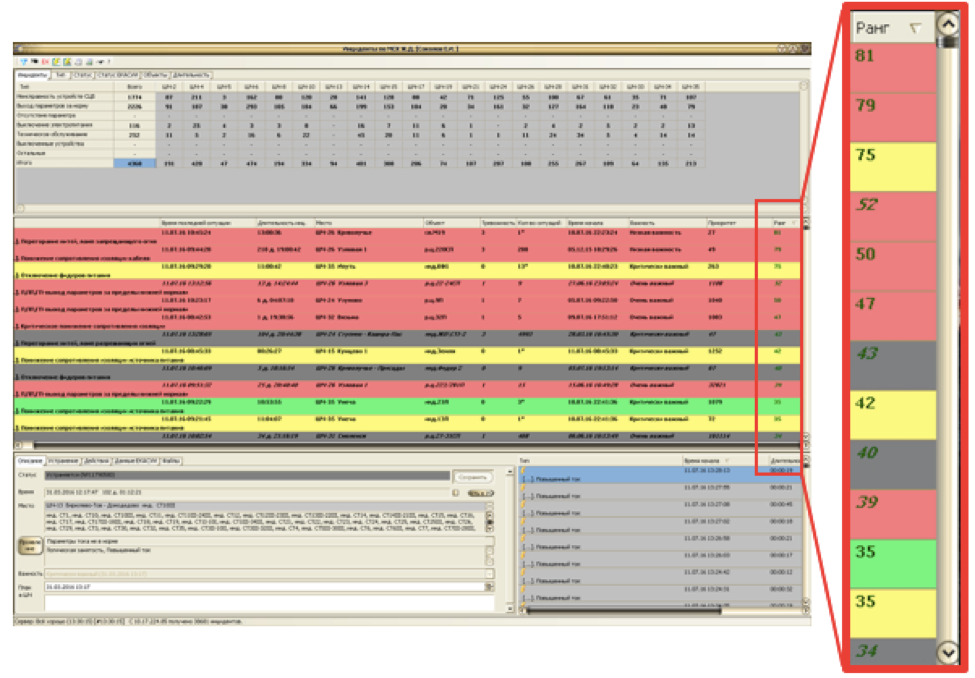
\includegraphics[width=10cm]{ui}
\caption{Отображение результатов ранжирования в пользовательском интерфейсе инженера службы мониторинга.}
\centering
\label{fig:ui}
\end{figure*}

Построенная модель ранжирования инцидентов была интегрирована в виде нового элемента, АПК «САРИ» (Система автоматического ранжирования инцидентов), в комплекс диспетчерского контроля ЦУСИ РЖД. Схема интеграции и взаимодействующие модули представлены на рис. \ref{fig:modules}.

Модуль ранжирования инцидентов выполняется на изолированном сервере. Он синхронно опрашивает модуль хранимых процедур в базе данных инцидентов на предмет обновления полей инцидентов и при необходимости инициирует пересчет при получении новых инцидентов и ситуаций. Важно отметить, что не все поля данных могут быть получены в оперативном режиме.

При получении новых данных, модуль осуществляет ранжирование инцидентов по набору исходных признаков и выдает прогнозное значение. Это значение далее отображается в виде отдельного столбца в интерфейсе инженера службы мониторинга с возможностью сортировки, см. рис. \ref{fig:ui}. Предсказательная модель выдает обновленное ранжирующее значение за 1.2 миллисекунды. Для удобства восприятия операторами, ранги инцидентов выдаются в виде целых чисел из интервала $[0,100]$ и соответствуют интервалу вероятностей $[10^{-6},1]$ на логарифмической шкале.


На исторических данных построено решающее правило, лес из 4000 решающих деревьев глубины 10.  Итоговое правило имеет 300,549 вариантов исходов и включает в себя более 3 лет исторических данных (5.3 млн инцидентов).

За время подконтрольной эксплуатации системы (май--июнь 2016 года, 1 месяц) в ней было зарегистрировано 581 032 ситуаций, объединенных в 92 339 инцидентов. Среди них предотказами было признано 2187 инцидентов. %Среднее время ответа САРИ – 1.7 мс.
Точность модели в тестовой эксплуатации оказалась очень близка к предварительной оценке на тестовой выборке (AUC 0.901 и 0.904, соответственно).

\begin{figure}
\centering
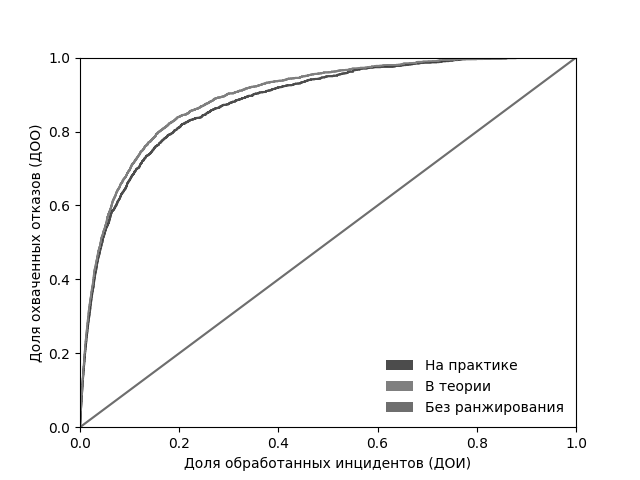
\includegraphics[width=10cm]{image19}
\caption{Операционная характеристика функции ранжирования (в теории и на практике)}
\centering
\label{fig:image19}
\end{figure}

На практике была показан режим работы, при котором для захвата 80\% предотказов достаточно охватить 20\% общей массы инцидентов в системе. Оценка снижения времени реакции инженера мониторинга на предотказ - до 5 раз (см. Рис. \ref{fig:ROCcurves}).

Модель полезно периодически обновлять, чтобы учитывать свежие данные. На графике ниже показано улучшение при обновлении раз в квартал.
Содержание главы опубликовано в работах:~\cite{itivs-2017} ~\cite{bulletin-rzd}.



\underline{\textbf{В третьей главе}} «Анализ и построение системы управления сетью малых базовых станций пятого поколения» исследуются способы максимизации суммарной пропускной способности сети базовых станций с обеспечением честности распределения ресурсов между пользователями за счет управления мощностью передачи в реcурсных блоков. Пиковая пропускная способность пользователя $k$, обслуживаемого в ресурсном блоке $n$ базовой станции $i$ задается следующим образом:

\begin{equation}
    \label{eq:throughput}
    \rho_{k,i,n} = \log \left(1 + \frac{\pi_{i,n} G_{k,i,n}}{N_0 + \sum_{i'\neq i}{\pi_{i',n} G_{k,i',n}}}\right)
\end{equation}

Обозначим за $\theta_{k,n}$ процент времени, занимаемый пользователем $k$ в ресурсном блоке $n$. Таким образом, средняя пропускная способность для пользователя задается следующим выражением~(\ref{eq:uthroughput}):

\begin{equation}
    \label{eq:uthroughput}
    \sum_{n \in \mathcal{N}} \theta_{k,n} \cdot \rho_{k,i,n}
\end{equation}

Задачу оптимизации для рассматриваемого сценария можно сформулировать следующим образом. Целевая функция $\eta(\pi, \theta)$ состоит из суммы логарифмов показателей пропускной способности для обслуживаемых пользователей.

\begin{equation}
\label{eq:maximize}
\eta = \sum_{i \in \mathcal{I}} \sum_{k \in \mathcal{K}(i)} \log \left(\sum_{n \in \mathcal{N}} \theta_{k,n} \cdot \log \left(1 + \frac{\pi_{i,n} G_{k,i,n}}{N_0 + \sum_{i'\neq i}{\pi_{i',n} G_{k,i',n}}}\right)\right)
\end{equation}

Такая структура целевой функции $\sum_{k=1}^K \log(r_k)$ (см.~(\ref{eq:maximize})) традиционно используется для максимизации суммарной пропускной способности в системах с $K$ пользователями для достижения справедливости распределения ресурсов. Может быть показано, что для решения $r^* = (r_1,r_2,...,r_K), r^* \in \Lambda$ задачи максимизации справедливо  неравенство (\ref{eq:propfairness}),  совпадающее с определением \textit{пропорционально справедливого} распределения ресурсов между $K$ пользователями~\cite{ETT:ETT4460080106}.

\begin{equation}
\label{eq:propfairness}
\sum_{k=1}^K \frac{r_k - r_k^*}{r_k^*} \leq 0, \forall r \in \Lambda
\end{equation}

Задача максимизации фукционала $\eta$ дополняется следующими ограничениями: выражения~(\ref{eq:limitationsa})--(\ref{eq:limitationsc}) гарантируют, что ресурсный блок не используется повторно сразу несколькими пользователями одной базовой станции,  ограничения~(\ref{eq:limitationsd})~и~(\ref{eq:limitationse}) соответствуют физическим ограничениям на суммарную мощность передачи по всем ресурсным блокам и минимальной мощности передачи в отдельном ресурсном блоке.

\begin{subequations}
\begin{equation}
\label{eq:limitationsa}
\sum_{k \in \mathcal{K}(i)} \theta_{k,n} \leq 1, \forall n \in \mathcal{N}
\end{equation}

\begin{equation}
\label{eq:limitationsb}
\sum_{n \in \mathcal{N}} \theta_{k,n} \leq 1, \forall k \in \mathcal{K}(i)
\end{equation}

\begin{equation}
\label{eq:limitationsc}
0 \leq \theta_{k,n} \leq 1, \forall k \in \mathcal{K}(i), \forall n \in \mathcal{N}
\end{equation}

\begin{equation}
\label{eq:limitationsd}
\sum_{n \in \mathcal{N}} \pi_{i,n} \leq P_{max}, \forall i \in \mathcal{I}
\end{equation}

\begin{equation}
\label{eq:limitationse}
\pi_{i,n} \geq \pi_{min}, \forall i \in \mathcal{I}, \forall n \in \mathcal{N}
\end{equation}
\end{subequations}

%\subsection{Декомпозиция оптимизационной задачи}
Для упрощения была показана возможность разделить задачу максимизации фукционала~(\ref{eq:maximize}) на две независимые задачи оптимизации - задачу распределения ресурсов между пользователями и задачу управления мощностью в ресурсных блоках. Воспользуемся неравенством для выпуклой функции ($f\left(\sum _{{i=1}}^{{n}}q_{i}x_{i}\right)\leq \sum _{{i=1}}^{{n}}q_{i}f(x_{i})$), чтобы получить нижнюю оценку для целевой функции $\eta$:

\begin{equation}
    \label{eq:jensen}
    \log{\sum_{n \in \mathcal{N}} \theta_{k,n} \cdot \rho_{k,i,n}} \geq \frac{\sum_{n \in \mathcal{N}} \log{\theta_{k,n} \cdot \rho_{k,i,n}}}{|\mathcal{N}|} + \log{|\mathcal{N}|}
\end{equation}

Таким образом для получения нижней оценки максимума функции $\eta(\pi, \theta)$ (см. формулу ~(\ref{eq:maximize})) предлагается производить оптимизацию функционала $\eta'$ с ограничениями ~(\ref{eq:limitationsa})--(\ref{eq:limitationse}). В такой постановке задачу оптимизации возможно разделить на две независимые задачи - задачу распределения ресурсов между пользователями и задачу управления мощностью в ресурсных блоках.

\begin{equation}
\label{eq:maximizealt}
\eta' = \sum_{i \in \mathcal{I}} \sum_{k \in \mathcal{K}(i)} \sum_{n \in \mathcal{N}} (\log(\theta_{k,n}) + \log( \rho_{k,i,n}))
\end{equation}

\begin{figure}
    \centering
    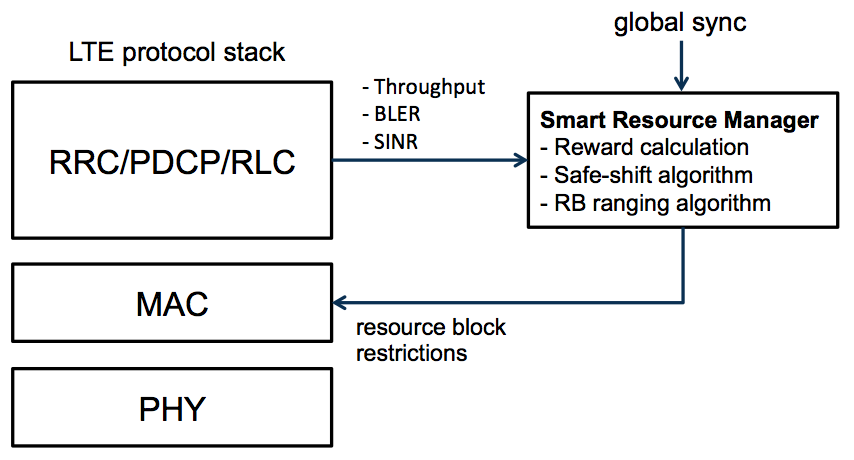
\includegraphics[width=8cm]{gcimages/algo_arch}
    \caption{Структура алгоритма и место в стеке протоколов LTE: PHY - физический уровень, MAC - уровень управления доступом к среде, RRC/PDCP/RLC - верхние уровни стека LTE}
    \label{fig:algo_arch}
\end{figure}

На Рис.~\ref{fig:algo_arch} представлена упрощенная структура алгоритма в стеке протоколов сети LTE. Можно заметить, что входящие или исходящие каналы управления не используются. Таким образом предлагаемое решение не налагает каких-либо требований на качество канала между базовыми станциями и выполняется локально на каждой малой соте.
Общий принцип алгоритма заключается в следующем. Основываясь на статистике производительности слоя L2~\cite{TS36.300} (например, BLER, спектральная эффективность) каждая малая сота локально принимает решение об использовании ресурсных блоков на последующем периоде времени. Единственный внешний входящий канал управления - глобальный источник точного времени. Он используется для выполнения синхронных операций (безопасный сдвиг) в пределах группы малых сот. После принятия решения о распределении ресурсов в каждой соте, выбранные ресурсные блоки  распределяются между пользователями базовой станции на уровне доступа к среде.

%\subsection{Схема распределения радиоресурсов}
В этой части мы рассмотриваем разнородные сети LTE состоящие из множества малых сот, сосуществующих с окружающими базовыми макро станциями. Базовые макро станции и малые соты работают в одном частотном диапазоне, чтобы увеличить повторное использование пространственной частоты.

Для координации интерференции между соседними сотами каждая малая сота автономно принимает решения о распределении частот. Весь доступный частотный диапазон разбивается на ряд поддиапазонов $b_{j}$, где $j=1, .., N$ и $N$ - общее количество поддиапазонов. Распределение ресурсов внутри каждой базовой станции осуществляется планировщиком с алгоритмом пропорционального справедливого разделения (англ. Proportional fair).

В момент времени $t$ автономный агент должен решить, какой поддиапазон $b(t+1)$ из имеющегося спектра доступен для использования на следующем временном промежутке $t+1$. Мы предлагаем схему обучения, состоящую из двух уровней (см. Рис.~\ref{fig:algo_arch}):

\begin{itemize}
\item[$\cdot$] параллельное обучение с подкреплением~\cite{4445757}, с $N\times N$ матрицей перехода $T(t)$. Она определяет вероятность перехода агента из поддиапазона $i$ в поддиапазон $j$ в момент времени $t$. Элементы матрицы периодически обновляются полученными наградами $RW_{ij}(t) = e^{(C_i(t-1) - C_j(t))}$, где $C_j(t)$ - достигаемая пропускная способность или количество пользователей с удовлетворенными требованиями к качеству обслуживания в момент времени $t$ при использовании поддиапазона $j$.
\item[$\cdot$] исследование макросреды (см. разд.~\ref{sec:safe_shift}), верхний уровень алгоритма с исследованием макросреды без вмешательства, где обучаемые агенты синхронно выполняют согласованную смену схемы использования ресурсов (безопасный сдвиг). $RW_{ij}(t_{sh})$ рассчитывается точно так же, как $RW_{ij}(t)$, но во время этапа безопасного сдвига. Этот шаг отвечает за обеспечение сосуществования с невзаимодействующими агентами и исследования макросреды.
\end{itemize}

Матрица перехода $T$ определяет вероятность перехода из поддиапазона $i$ к поддиапазону $j$. Значения $T_{ij}(t)$ и $T_{ij}(t_{sh})$ обновляются на каждой итерации (каждую 1 мс) на основе функции вознаграждения как описано в~(\ref{eq:tm_update}).
\begin{equation}
    \label{eq:tm_update}
    T_{ij}(t) = (1-\alpha-\beta)T_{ij}(t-1) + \alpha RW_{ij}(t) + \beta RW_{ij}(t_{sh})
\end{equation}
\begin{equation}
    \label{eq:tm_update_c}
    RW_{ij}(t) = e^{(C_i(t-1) - C_j(t))}
\end{equation}
где:

\begin{itemize}
\item[$\cdot$]$ \alpha$ - коэффициент обучения, определяющий скорость сходимости алгоритма и соотношение этапов исследования и эксплуатации. Оптимальное значение для этого параметра подбирается экспериментально в ходе симуляций.
\item[$\cdot$] $\beta$ - коэффициент обучения ($\beta < \alpha$) для макросреды, определяющий скорость сходимости алгоритма верхнего уровня.
\end{itemize}

В то время как соты не имеют одинаковых знаний об уровне занятости/интерференции каждого поддиапазона, матрица перехода $T$ обновляется независимо для каждой соты. В определенной степени, это может привести к уменьшению скорости сходимости алгоритма. Моделирование показывает, что этим поведением можно эффективно управлять с помощью тонкой настройки коэффициентов обучения. Далее показан дополнительный метод для повышения скорости сходимости алгоритма.

%\subsection{Исследование макросреды: алгоритм безопасного сдвига}
\label{sec:safe_shift}
Любой агент в каждый момент времени наблюдает ответ окружающей среды $\gamma = \gamma^{CL} + \gamma^{ML}$, который состоит из двух частей: $\gamma^{CL}$ - компонент, определяемый поведением соседних агентов, а $\gamma^{ML}$ - независимый компонент, определяемый слоем макросреды.
Существует простой случай так называемой блокировки канала, где этап исследования окружающей среды $\gamma^{ML}$ агентом №2 заблокирован компонентой $\gamma^{CL}$, обусловленной выбором диапазона агента №1. Аналогичным образом на практике подавляющее большинство попыток разведки будут заблокированы ответом канала $\gamma_b^{CL}$ соседей.

Чтобы побороть описанный эффект мы заставляем каждого агента изучать ответ макросреды $\gamma_b^{ML}$ в пределах каждого параллельного этапа обучения $t$ - процедуры безопасного сдвига. В рамках этой процедуры каждый агент последовательно изучает поддиапазоны в следующем порядке: ${(b_{t+1}+i)~mod~N}, i=1..N$. Очевидно, что это изменение не повлияет на компонент ответа $\gamma^{CL}$, так как агенты на пересекающихся поддиапазонах в момент времени $t$ по-прежнему используют те же поддиапазоны в момент времени ${t+1}$. В то же время компонент $\gamma^{ML}$ базового ответа окружающей среды изменяется.

Изучая отличия ответов окружающей среды $\gamma_b$, мы можем скорректировать оценки величин $\gamma_b^{ML}$ и $\gamma_b^{CL}$ для каждого агента в отдельности. Чтобы сохранить свойство локальности алгоритма, мы предлагаем управлять моментом запуска процедуры безопасного сдвига для каждого агента при помощи источника глобального времени. Значения функции вознаграждения при процедуре безопасного сдвига учитываются в соответствующей статистике для поддиапазонов в качестве отдельного компонента (см. формулу~\ref{eq:tm_update}). В результате обновления условия $\beta RW_{ij}(t_{sh})$, обучаемые агенты должны выбрать поддиапазоны с лучшим ответом макросреды.

Следующий эксперимент иллюстрирует простой пример процедуры безопасного сдвига. Рассмотрим случай двух малых сот разделяющих два частотных поддиапазона, где один из поддиапазонов занят невзаимодействующим агентом (например, базовая макро станция). После схождения процесса обучения малые соты 1 и 2 используют подздиапазоны 2 и 1 соответственно, каналы блокируются для исследования. Пусть поддиапазон 1 также занимает базовая макро станция или невзаимодействующий агент. Результат влияния процедуры безопасного сдвига на общую пропускную способность сети представлен на рис.~\ref{fig:safe_shift_overal_throughput}, где сдвиги производятся в моменты времени $t_1=200$ мс и $t_2=400$ мс. Этот шаг не влияет на взаимную интерференцию между агентами, но измененяет уровень помех от макросреды. Прирост около $10\%$ достигается без необходимости возобновления параллельного обучения для обоих агентов.

\begin{figure}
    \centering
    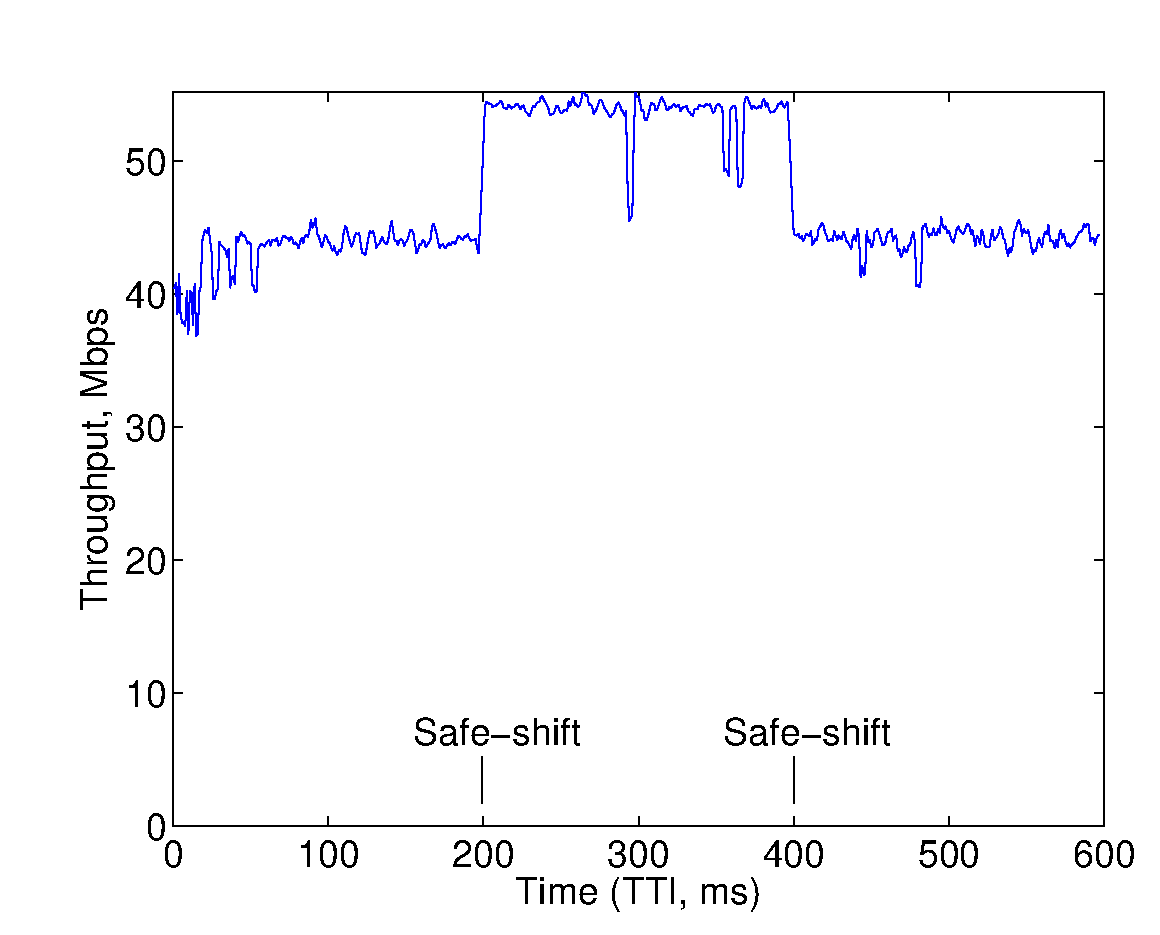
\includegraphics[width=8cm]{gcimages/overal_throughput}
    \caption{Прирост пропускной способности. Процедура безопасного сдвига инициирована в моменты времени $t_1=200$ мс и $t_2=400$ мс }
    \label{fig:safe_shift_overal_throughput}
\end{figure}

%\subsection{Исследование скорости сходимости, выкалывание множества состояний}
В процессе обучения агенты постоянно изменяют свое состояние. Это в свою очередь инвалидирует стратегии других агентов, делая исходные условия, на которых они построены, устаревшими. Общий подход к этой проблеме заключается в том, чтобы считать этот эффект частью динамично изменяющейся среды. Однако, это предположение ослабляется в случае параллельного обучения множества агентов, где поведение динамической среды в большей степени определяется самими агентами.
Для того, чтобы преодолеть определяющую роль случайного исследования в структуре окружающей среды, мы предлагаем следующий способ. Идея в том, чтобы предварительно заставить агентов вести себя уникальным образом. В этом случае даже в процессе обучения посредством случайного исследования агенты могли бы получать статистически значимые наблюдения о поведении соседних агентов. Для этого мы предлагаем случайно выколоть часть $p$ $(p< 1)$ элементов матрицы перехода $TM_{ij}$ для каждого агента. Ожидается, что этот метод значительно уменьшит время сходимости процесса обучения.

Представим себе изменение поведения значения скорости сходимости в зависимости от параметра $p$ (показания усредненны для случайного набора из 500 прогонов иммитационной модели). Под скоростью сходимости понимается отношение продолжительности этапа эксплуатации к общей продолжительности работы системы. Значение $p = 0$ соответствует случаю, когда на переходные правила не накладывается никаких ограничений. Значение $p>0$ - конфигурации, когда некоторая часть переходов случайным образом запрещена для каждого агента. Видно, что для определенных значения коэффициент сходимости увеличивается до $20\%$.
Содержание главы опубликовано в работах ~\cite{5G},~\cite{globecom},~\cite{ent-2017}.

% \subsection{Channel blocking}



В \underline{\textbf{четвертой главе}} «Разработка специального математического и алгоритмического обеспечения систем обработки информации в эргатических системах» приведено описание
\todo{Четвертая глава сведение воедино, те самые методические указания}
\todo{Опишем все внедрения + типовой проект, как шел проект с ржд, календарный план и этапность работ в проекте ржд. Подход к решению задачи nlp подход к решению задачи по турбинам, предполагаемый подход к решению задачи по киберакадемии}
\todo{Описание оргструктуры проекта от Быкова (по РЖД)}
\todo{Философия из чужой диссертации по РЖД}
\todo{Работа по ГОСТам 19, 26}
\todo{Содержание главы опубликовано в работах}


В \underline{\textbf{заключении}} приведены основные результаты работы, которые заключаются в следующем:
%% Согласно ГОСТ Р 7.0.11-2011:
%% 5.3.3 В заключении диссертации излагают итоги выполненного исследования, рекомендации, перспективы дальнейшей разработки темы.
%% 9.2.3 В заключении автореферата диссертации излагают итоги данного исследования, рекомендации и перспективы дальнейшей разработки темы.
применение машинного обучения приносит свои плоды, однако внедрение затруднено тем, что клиенты не готовы доверять автоматизированным системам такого уровня абстракций. Трактовка работы моделей на базе машинного обучения и визуализация результата является необходимой частью успешного проекта. При этом желательно, чтобы трактовка происходила в реальном времени, с привлечением экспертов рабочей группы с самого начала разработки системы.
Опыт применения методов машинного обучения к задачам управления инфраструктурой российских железных дорог на Московской железной дороге  позволяет  ожидать  положительные  практические результаты при дальнейшем развитии и тиражировании достигнутых совместной рабочей группой специалистов.
По  результатам  доклада  генерального  директора  компании  ООО «Телум»  Павла  Бойко, Ученый  совет  ОАО «РЖД»  признал  перспективным применение современных методов машинного обучения к задачам управления инфраструктурой российских железных дорог и порекомендовал продолжить развитие, разработку и внедрение си-стемы в составе более широкой совместной груп-пы, с вовлечением отраслевых институтов и университетов (в т.ч. АО«ВНИИЖТ»). Представленные наработки в области интеллектуального анализа данных также рекомендовано апробировать в других областях железнодорожного транспорта.
\begin{enumerate}
  \item \todo{На основе анализа \ldots}
  \item \todo{Численные исследования показали, что \ldots}
  \item \todo{Математическое моделирование показало \ldots}
  \item \todo{Для выполнения поставленных задач был создан \ldots}
\end{enumerate}



%\newpage
% При использовании пакета \verb!biblatex! список публикаций автора по теме
% диссертации формируется в разделе <<\publications>>\ файла
% \verb!../common/characteristic.tex!  при помощи команды \verb!\nocite!

\ifdefmacro{\microtypesetup}{\microtypesetup{protrusion=false}}{} % не рекомендуется применять пакет микротипографики к автоматически генерируемому списку литературы
\ifnumequal{\value{bibliosel}}{0}{% Встроенная реализация с загрузкой файла через движок bibtex8
  \renewcommand{\refname}{\large \authorbibtitle}
  \nocite{*}
  \insertbiblioauthor                          % Подключаем Bib-базы
  %\insertbiblioother   % !!! bibtex не умеет работать с несколькими библиографиями !!!
}{% Реализация пакетом biblatex через движок biber
  \insertbiblioauthor                          % Подключаем Bib-базы
  \insertbiblioother
}
\ifdefmacro{\microtypesetup}{\microtypesetup{protrusion=true}}{}
